\chapter{Design}
In diesem Kapitel geht es darum die Vor- und Nachteile der unterschiedlichen
Bibliotheken anhand eines praktischen Beispieles zu zeigen. Dabei wird
\enquote{gelly-streaming} als Referenz-Implementierung benutzt. Zunächst wird
allgemein der Ablauf des Beispiel beschrieben. Dann wird die Architektur
der Referenz beschrieben. Anschließend werden die Entwürfe für die anderen
Bibliotheken beschrieben und was die Besonderheiten in Bezug auf die Referenz
sind. Abschließend werden die Probleme der Bibliotheken benannt und mögliche
Lösungsmöglichkeiten benannt.

\section{Analyse des Beispieles}
In dem Beispiel geht es darum zu überprüfen, ob ein Graph bipartite ist oder
nicht. Dies bedeutet, ob ein Graph zweifarbig färbbar ist. Um dies für einen
existierenden Graphen zu lösen, gibt es verschiedene Algorithmen. Die allgemeine
Vorgehensweise ist dabei ähnlich.

Am Begin sind alle Knoten ungefärbt. Dann werden zwei Farben gewählt.
Anschließend wird ein Startknoten gewählt und dieser in einer der Farben markiert.
Dann werden die unmarkierten Nachbarknoten in der anderen Farbe markiert. Danach
werden deren unmarkierte Nachbarknoten wieder in der ersten Farbe markiert, usw.
bis alle Knoten makiert sind. Ein Graph ist dann bipartite, wenn alle Knoten so
markiert sind, dass keine benachbarten Knoten die selbe Farbe haben. Diese
Vorgehensweise kann jeder selbst für kleine Graphen selbst durchführen. Je nachdem
welche Informationen über den zu überprüfenden Graphen existieren, kann der Ablauf
auch verkürzt werden. Wenn der Graph nämlich einen Kreis von ungerader Länge
enthällt ist, kann der Graph nie bipartite sein unabhängig vom gewählten
Startknoten. Die Abbildung \ref{fig:bipartite-six-nodes} zeigt einen bipartiten
Graphen mit einen Kreis der Länge sechs. Während dessen die Abbildung \ref{fig:bipartite-five-nodes}
einen nicht bipartiten Graphen zeigt. Denn der Kreis hat eine ungerade Länge und
lässt sich damit nie mit zwei Farben färben egal welcher Startknoten gewählt
wurde. 

\begin{figure}
\centering
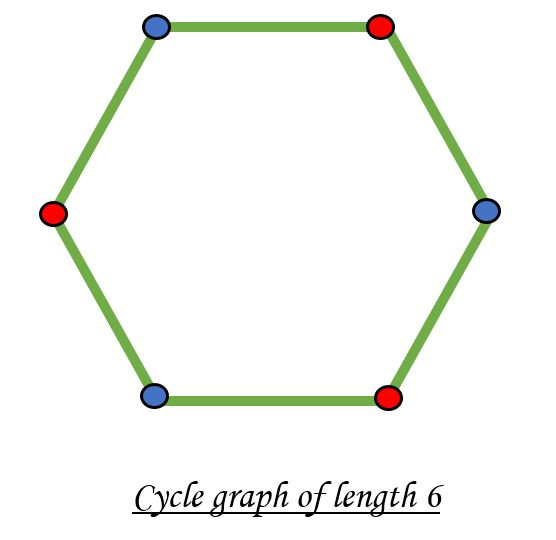
\includegraphics[scale=0.5]{../material/images/bipartite-graph-six-nodes.jpg}
\caption{bipartiter Graph mit Kreis der Länge sechs \cite{GeeksforGeeks2018}}
\label{fig:bipartite-six-nodes}
\end{figure}

\begin{figure}
\centering
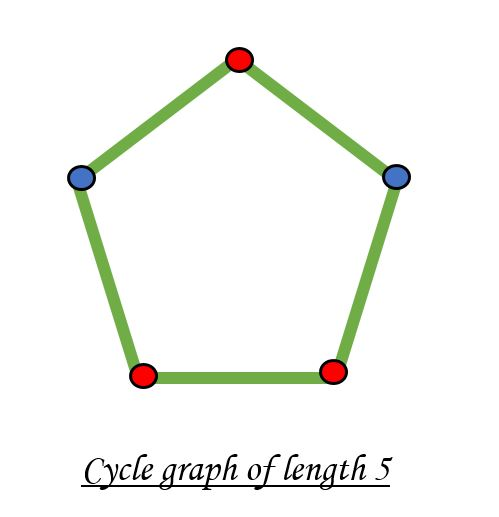
\includegraphics[scale=0.5]{../material/images/bipartite-graph-five-nodes.jpg}
\caption{nicht bipartiter Graph mit Kreis der Länge fünf \cite{GeeksforGeeks2018}}
\label{fig:bipartite-five-nodes}
\end{figure}


Wie läuft das Beispiel nun konkret ab. Zunächst werden die Daten eingelesen. Dies
erfolgt zur Vereinfachung über eine Datei. Dies kann jedoch jederzeit auf eine
alternative Eingabe umgestellt werden zum Beispiel um die Daten von einem
Messaging-System wie Apache Kafka einlesen zu können. Dabei ist zu beachten,
dass alle Bibliotheken, verschiedene Eingabeformate haben. Anschließend werden
die Daten an eine beliebige Ausgabe gesendet. Dies ist in unserem Fall einfach
die Konsole.

\subsection{Architektur der Referenz-Implementierung}
Die Anwendung besteht aus drei Teilen, welche wie eine Fileterkette aufgebaut
sind Eingabe, Verarbeitung und Starten. Alle drei Teile definieren einen Apache
Flink Job und in jede Anwendung sollte maximal nur einen Job umsetzen. Zunächst
muss die Streaming-Engine initialisiert werden. Dabei ist es von Vorteil, zu
wissen ob die spätere Anwendung nur lokal oder remote betrieben werden soll.
Lokal bedeutet in diesem Zusammmenhang, dass die Anwendung einen Apache Flink
Cluster in der selben JVM startet. Dies lässt sich bereits bei der Entwicklung
fest einzuprogrammieren oder dynamisch von Apache Flink bestimmen lassen.

\foreigntextquote{english}[\cite{Foundation2018}]{
The LocalStreamEnvironment is a StreamExecutionEnvironment that runs the program
locally, multi-threaded, in the JVM where the environment is instantiated. It
spawns an embedded Flink cluster in the background and executes the program on
that cluster.}

Danach können die eigentlichen Daten eingelesen werden. Dazu kann ein von Apache
vordefinierter Connector zum Beispiel für Dateien benutzt werden oder eine
Bibliothek. In diesem Beispiel wird der File-Connector benutzt, welcher im Kern
von Apache Flink enthalten ist. Die Umwandlung von Text zu Kanten muss für jede
Anwendung neu definiert und programmiert werden. Im Beispiel liegen die Daten
wie schon erwähnt in einer Datei vor. Dabei besteht jede Zeile aus genau einer
Kante. Jede Kante besteht dabei aus zwei Identifikationsnummern für die Kanten,
welche durch ein Tabulator getrennt sind. Alle Kanten sind in Apache Flink
gerichtete Kanten. Eine ungerichtete Kante kann nur erzeugt werden, wenn es eine
zweite Kante gibt, bei der die Anfangs- und End-Identifikationsnummern vertauscht
sind.

\foreigntextquote{english}[\cite{Foundation2018}]{
In Gelly an Edge is always directed from the source vertex to the target vertex.
A Graph may be undirected if for every Edge it contains a matching Edge from the
target vertex to the source vertex.}

Anschließend erfolgt die richtige Datenverarbeitung bei der das Filter-Pattern
zur Anwendung kommt, wie es auch bei anderen Anwendungen, wie Map-Reduce zum
Einsatz kommt. Dabei wird auch die Ausgabe mit definiert. Im Beispiel wird der
Graph dann überprüft, ob dieser bipartite ist oder nicht. Dabei werden die Daten
in einem temporären Stream mit Fenster zwischengespeichert. Die Überprüfung wird
in eine Aggretationsfunktion eingebettet um die Zwischenergebnisse zu speichern.
Als letztes wird der Job dann gestartet. Dabei wird in der lokalen Umgebung dann
der Cluster gestartet.

\subsection{Entwurf von \enquote{graphstream-project}}
Die Umsetzung des Beispiel ist ähnlich wie eine normale Java-Anwendung zu
programmieren. Zunächst wird die Eingabe definiert. In \enquote{graphstream-project}
sind werden Eingabe-Komponenten als \enquote{Sources} bezeichnet. Hier in diesem
Beispiel werden die Graphendaten wieder von einer Datei bereitgestellt. Die
Bibliothek stellt ein Protokoll zur Datenübertragung bereit. Dadurch ist eine
einfache Kommunikation auch mit anderen Systemen möglich. Das Protokoll hat dabei
Ähnlichkeiten zum \enquote{Portable Bitmap File} Format. Beide Protokolle haben
am Anfang einen Kopf für die Meta-Informationen bevor die eigentlichen Daten
folgen. Im Unterschied zu \enquote{gelly-streaming} lassen sich die Kanten
genau spezifizieren.

ae Allows to add an edge. This command must be followed by the unique identifier
of the edge, and then the identifiers of two other nodes. As for nodes, you can
specify a parameter list. It is possible to create directed edges by adding a
“>” (greater-than) or “<” (smaller-than) character between the nodes identifiers.
This indicates the direction of the edge. When no “<” or “>” is present, the
edge is not directed.

Die Quelle wird dann mit einer Graph-Instanz verbunden. Denn es ist möglich
den Graphen durch den Aufruf von Methoden zu ändern.

Die Implementierung von Algorithmen erfolgt bei \enquote{graphstream-project}
über das Interface Algorithm. Dieses stellt zwei Methoden bereit init und compute.
Die Methode init bekommt einen Graphen übergeben und initialisiert den
Algorithmus. Die compute Methode führt die eigentliche Berechnung aus.
Die Resultate des Algorithmus werden über selbst programmiert Getter
bereitgestellt.

Die Ausgabe erfolgt über einen Aufruf der Konsole.

\subsection{Entwurf von \enquote{Gephi}}

\section{Bewertung und Alternativen}

Bei der Ausführung des Beispiels fällt auf, dass für jede neue Kante ein
Ergebnis produziert wird. Dies sollte eigentlich nicht passieren, da ja ein
Fenster aktiv sein sollte und somit nur pro Fenster ein Ergebnis geliefert
werden sollte. Es kann natürlich daran liegen, dass die Daten aus einer Datei
eingelesen werden und nicht von einem Socket oder ähnliches.

Die Datenverarbeitung unterscheidet sich stark von der Referenz.
Bei \enquote{gelly-streaming} wird die Verarbeitung als Filterkette definiert,
welche dann von Apache Flink verwaltet wird. Der Aufruf der einelnen
Berechnungsschritte erfolgt dabei durch Apache Flink. Bei
\enquote{graphstream-project} müssen die einelnen Berechnungsschritte impliziet
aufgerufen werden. 

Interface Algorithm(Marker Interface) <-> Getter

